\documentclass{article} % \documentclass{} is the first command in any LaTeX code.  It is used to define what kind of document you are creating such as an article or a book, and begins the document preamble
\usepackage[left=1in, right=1in, top=0.5in, bottom=0.5in]{geometry}
\usepackage{graphicx}
\usepackage{amsmath} % \usepackage is a command that allows you to add functionality to your LaTeX code
\usepackage{subcaption}
\usepackage{ifthen}
\usepackage{xparse}
\usepackage{fancyvrb}
\usepackage{amsfonts}
\usepackage[export]{adjustbox}
\usepackage{float}
\parindent=0pt % disables indentation

\graphicspath{{../results/}{../writeup/}} 
\newcommand{\img}[3][0.3]{    
    \begin{figure}[H]
        \centering
        \includegraphics[width=\textwidth,keepaspectratio=true,height=#1\textheight]{#2}
        \caption{#3}
    \end{figure}
}
\newcommand{\imgl}[4][0.3]{    
    \begin{figure}[H]
        \centering
        \includegraphics[width=\textwidth,keepaspectratio=true,height=#1\textheight]{#2}
        \caption{#3}
        \label{#4}
    \end{figure}
}

\title{\large COMP5421 Computer Vision
\\ \huge Homework Assignment 5
\\ \huge Lucas-Kanade Tracking and Correlation Filters} 
\author{Hartanto Kwee Jeffrey\\
    \normalsize jhk@connect.ust.hk | SID: 20851871} % Sets authors name
\date{}

% The preamble ends with the command \begin{document}
\begin{document} % All begin commands must be paired with an end command somewhere
    \maketitle % creates title using information in preamble (title, author, date)
    
    \section[1]{Lucas-Kanade Tracking} % creates a section

    \subsection*{Q1.1}

    We are given the wrap function
    \begin{equation*}
    \mathcal{W}\left(x;p\right)=x+p
    \end{equation*}
    Hence,
    \begin{equation*}
    \frac{\partial \mathcal{W}(x;p)}{\partial p^{T}}=\frac{\partial }{\partial p^{T}}\left(x+p\right)=I_{2\times 2}
    \end{equation*}
    where $I_{2\times 2}$ is the identity matrix.
    \medskip

    Our objective function can hence be approximated as
    \begin{align*}
    &\arg \min _{\Delta p} \sum _{x}{\left| \left| \mathcal{I}_{t+1}\left(x+p+\Delta p\right)-\mathcal{I}_{t}\left(x\right)\right| \right| }_{2}^{2} \\
    \approx&\arg \min _{\Delta p} \sum _{x}{\left| \left| \mathcal{I}_{t+1}\left(x'\right)+\dfrac{\partial \mathcal{I}_{t+1}\left(x'\right)}{\partial x'^{T}}\Delta p-\mathcal{I}_{t}\left(x\right)\right| \right| }_{2}^{2}\\ 
    =&\arg \min _{\Delta p} \sum _{x}{\left| \left| \dfrac{\partial \mathcal{I}_{t+1}\left(x'\right)}{\partial x'^{T}}\Delta p-\left(\mathcal{I}_{t}\left(x\right)-\mathcal{I}_{t+1}\left(x'\right)\right)\right| \right| }_{2}^{2}\\ 
    =&\arg \min _{\Delta p} {\left| \left| A\Delta p-b\right| \right| }_{2}^{2}
    \end{align*}

    where $A=\left[\begin{array}{c}
    \dfrac{\partial \mathcal{I}_{t+1}\left({x}_{1}^{'}\right)}{\partial {x}_{1}^{'T}}\\
    \dfrac{\partial \mathcal{I}_{t+1}\left({x}_{2}^{'}\right)}{\partial {x}_{2}^{'T}}\\
    \vdots \\
    \dfrac{\partial \mathcal{I}_{t+1}\left({x}_{N}^{'}\right)}{\partial {x}_{N}^{'T}}
    \end{array}\right]$ and $b=\left[\begin{array}{c}
    \mathcal{I}_{t}\left(x_{1}\right)-\mathcal{I}_{t+1}\left({x}_{1}^{'}\right)\\
    \mathcal{I}_{t}\left(x_{2}\right)-\mathcal{I}_{t+1}\left({x}_{2}^{'}\right)\\
    \vdots \\
    \mathcal{I}_{t}\left(x_{N}\right)-\mathcal{I}_{t+1}\left({x}_{N}^{'}\right)
    \end{array}\right]$. Note that $A\in \mathbb{R}^{N\times 2}$, $\Delta p\in \mathbb{R}^{2}$ and $b\in \mathbb{R}^{N}$. For a unique solution of $\Delta p$ to be found, $A^{T}A$ should be non-singular.

    \subsection*{Q1.3}

    \begin{figure}[H]
        \centering
        \begin{subfigure}[b]{0.30\textwidth}
            \centering
            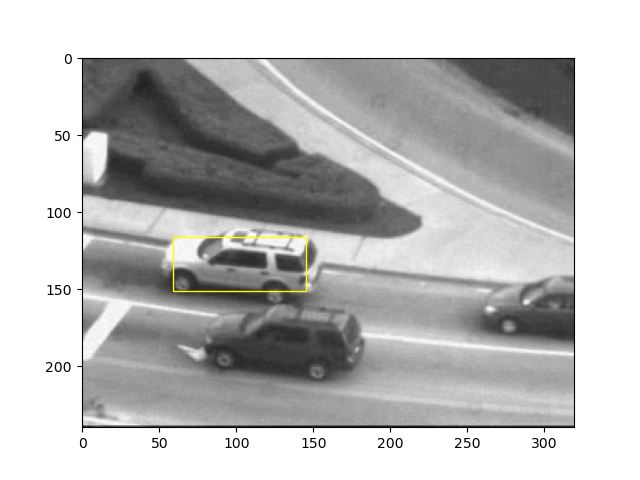
\includegraphics[width=\textwidth]{q1,3_frame0.png}
            \caption{Frame 0}
        \end{subfigure}
        \begin{subfigure}[b]{0.30\textwidth}
            \centering
            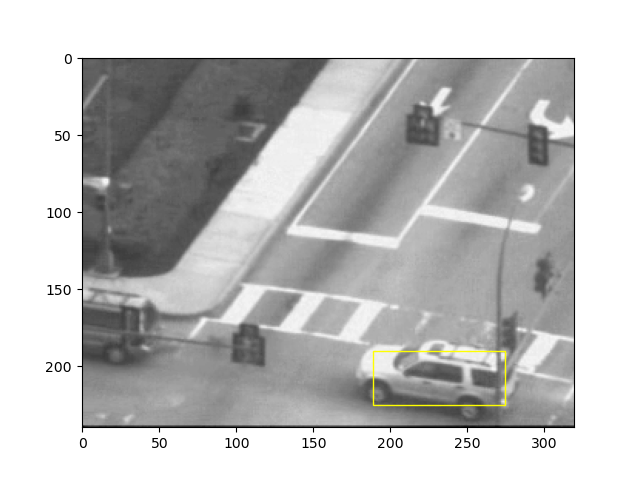
\includegraphics[width=\textwidth]{q1,3_frame100.png}
            \caption{Frame 100}
        \end{subfigure}
        \begin{subfigure}[b]{0.30\textwidth}
            \centering
            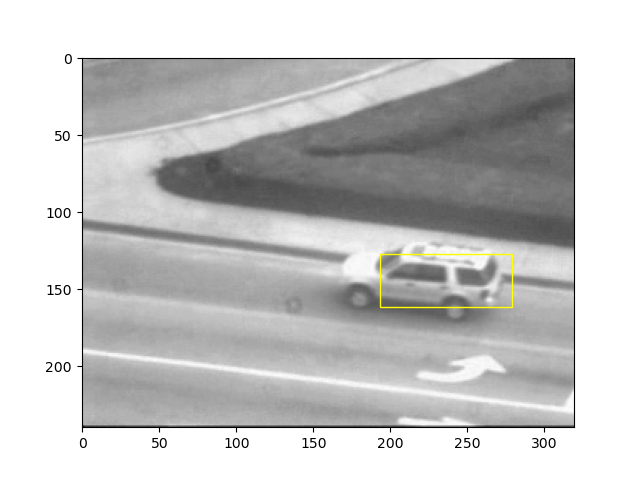
\includegraphics[width=\textwidth]{q1,3_frame200.png}
            \caption{Frame 200}
        \end{subfigure}
        \begin{subfigure}[b]{0.30\textwidth}
            \centering
            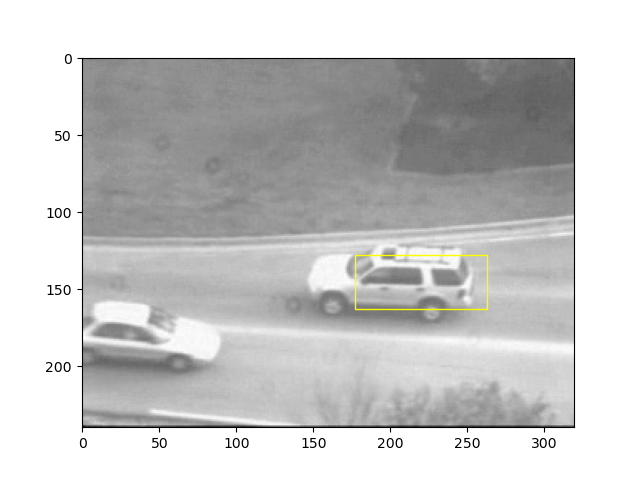
\includegraphics[width=\textwidth]{q1,3_frame300.png}
            \caption{Frame 300}
        \end{subfigure}
        \begin{subfigure}[b]{0.30\textwidth}
            \centering
            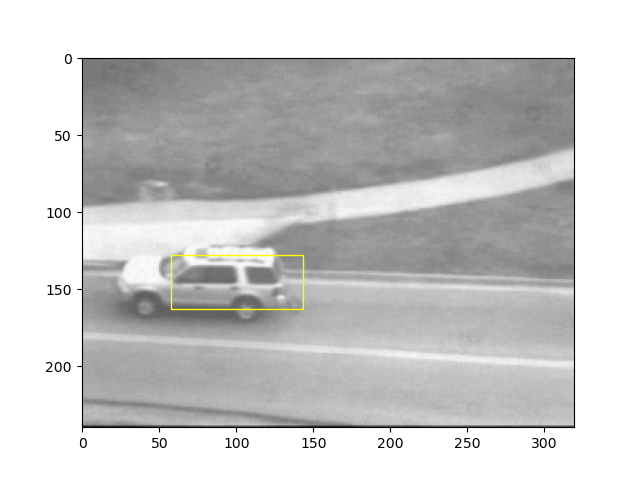
\includegraphics[width=\textwidth]{q1,3_frame400.png}
            \caption{Frame 400}
        \end{subfigure}
        \caption{Lucas-Kanade Tracking with One Single Template}
    \end{figure}

    \subsection*{Q1.4}
    \begin{figure}[H]
        \centering
        \begin{subfigure}[b]{0.30\textwidth}
            \centering
            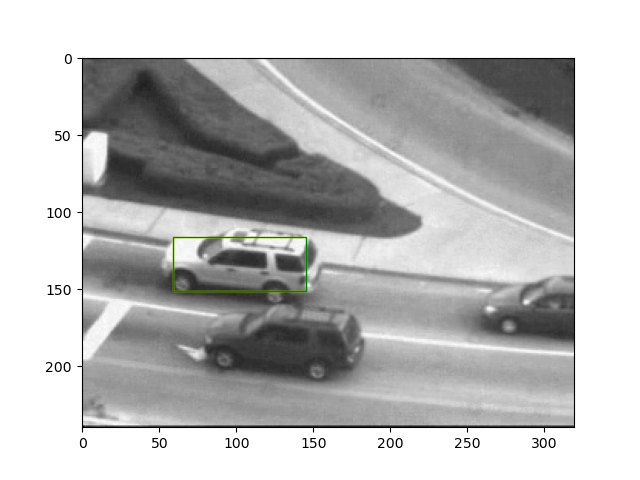
\includegraphics[width=\textwidth]{q1,4_frame0.png}
            \caption{Frame 0}
        \end{subfigure}
        \begin{subfigure}[b]{0.30\textwidth}
            \centering
            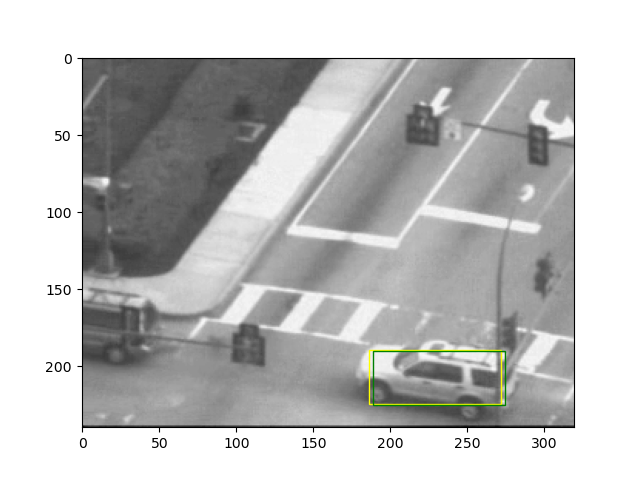
\includegraphics[width=\textwidth]{q1,4_frame100.png}
            \caption{Frame 100}
        \end{subfigure}
        \begin{subfigure}[b]{0.30\textwidth}
            \centering
            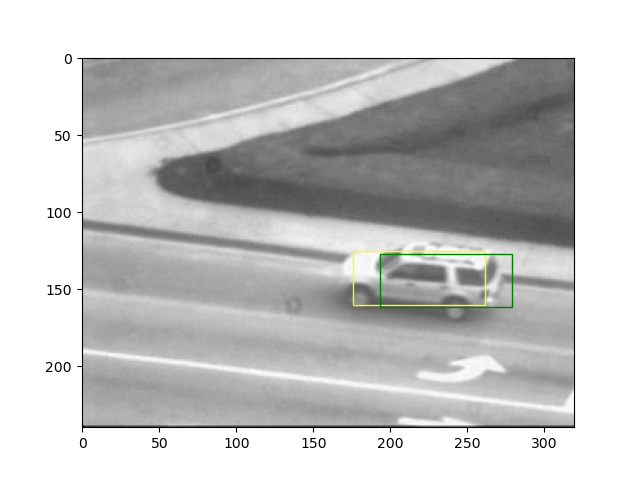
\includegraphics[width=\textwidth]{q1,4_frame200.png}
            \caption{Frame 200}
        \end{subfigure}
        \begin{subfigure}[b]{0.30\textwidth}
            \centering
            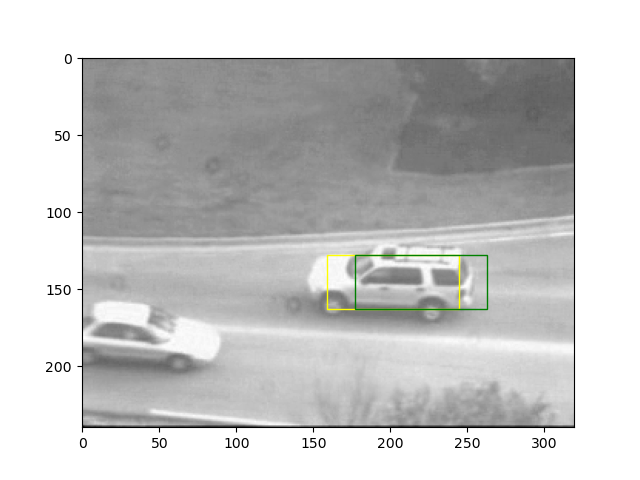
\includegraphics[width=\textwidth]{q1,4_frame300.png}
            \caption{Frame 300}
        \end{subfigure}
        \begin{subfigure}[b]{0.30\textwidth}
            \centering
            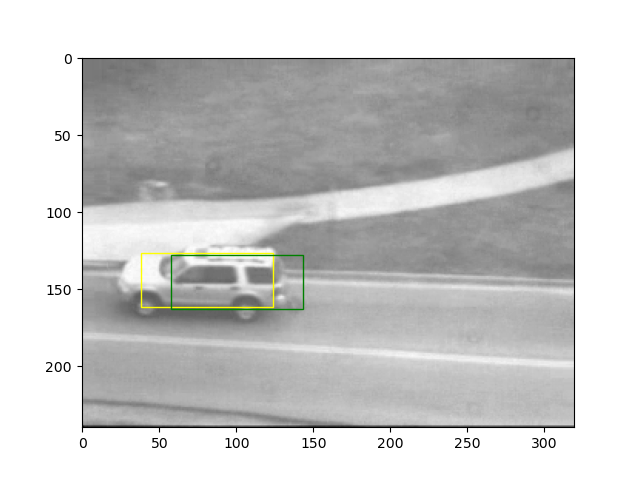
\includegraphics[width=\textwidth]{q1,4_frame400.png}
            \caption{Frame 400}
        \end{subfigure}
        \caption{Lucas-Kanade Tracking with Template Correction. The yellow bounding box is the result with template correction, and green one is the result without template correction.}
    \end{figure}

    \section{Appearance Basis}
    
    \subsection*{Q2.1}
    The previous and current frame are related by the following relationship:
    \begin{align*}
    \mathcal{I}_{t+1}\left(x\right)&=\mathcal{I}_{t}\left(x\right)+{\sum}_{k=1}^{K}w_{k}\mathcal{B}_{k}(x)\\
    \mathcal{I}_{t+1}\left(x\right)-\mathcal{I}_{t}\left(x\right)&={\sum }_{k=1}^{K}w_{k}\mathcal{B}_{k}(x)
    \end{align*}
    Since the basis for $B_{k}$ are orthogonal to each other, $\mathcal{B}_{i}\left(x\right)\cdot \mathcal{B}_{k}\left(x\right)=0$ if $i\neq k$. Therefore, to find $w_{i}$ for some $i$, we dot both sides with $\mathcal{B}_{i}(x)$:
    \begin{align*}
    \mathcal{B}_{i}\left(x\right)\cdot \left(\mathcal{I}_{t+1}\left(x\right)-\mathcal{I}_{t}\left(x\right)\right) & =\mathcal{B}_{i}\left(x\right)\cdot {\sum }_{k=1}^{K}w_{k}\mathcal{B}_{k}(x)\\ & =w_{i}\left(\mathcal{B}_{i}\left(x\right)\cdot \mathcal{B}_{i}\left(x\right)\right)\\
    w_{i} & =\frac{\mathcal{B}_{i}\left(x\right)\cdot \left(\mathcal{I}_{t+1}\left(x\right)-\mathcal{I}_{t}\left(x\right)\right)}{\mathcal{B}_{i}\left(x\right)\cdot \mathcal{B}_{i}\left(x\right)}
    \end{align*}
    Hence, $w=\left[\begin{array}{cccc}
    \dfrac{\mathcal{B}_{1}\left(x\right)\cdot \left(\mathcal{I}_{t+1}\left(x\right)-\mathcal{I}_{t}\left(x\right)\right)}{\mathcal{B}_{1}\left(x\right)\cdot \mathcal{B}_{1}\left(x\right)} & \dfrac{\mathcal{B}_{2}\left(x\right)\cdot \left(\mathcal{I}_{t+1}\left(x\right)-\mathcal{I}_{t}\left(x\right)\right)}{\mathcal{B}_{2}\left(x\right)\cdot \mathcal{B}_{2}\left(x\right)} & \ldots & \dfrac{\mathcal{B}_{K}\left(x\right)\cdot \left(\mathcal{I}_{t+1}\left(x\right)-\mathcal{I}_{t}\left(x\right)\right)}{\mathcal{B}_{K}\left(x\right)\cdot \mathcal{B}_{K}\left(x\right)}
    \end{array}\right]^{T}$.
    
    \subsection*{Q2.2}
    This section provides a derivation of the least squares form of the objective function for the gradient descent.
    \medskip
        
    We consider the new image as $\mathcal{I}_{t+1}\left(x+p\right)$. If ${\left\{\mathcal{B}_{k}\right\}}_{k=1}^{K}$ is an orthonormal basis, then $\mathcal{B}_{k}(x)\cdot \mathcal{B}_{k}(x)=1$. $w$ reduces to
    \begin{align*}
    w & =\left[\begin{array}{llll}
    \mathcal{B}_{1}\left(x\right) & \mathcal{B}_{2}\left(x\right) & \ldots & \mathcal{B}_{K}\left(x\right)
    \end{array}\right]^{T}\left(\mathcal{I}_{t+1}\left(x+p\right)-\mathcal{I}_{t}\left(x\right)\right)\\ & =\left[\begin{array}{llll}
    \mathcal{B}_{1}\left(x\right) & \mathcal{B}_{2}\left(x\right) & \ldots & \mathcal{B}_{K}\left(x\right)
    \end{array}\right]^{T}\left(A\Delta p-b\right)
    \end{align*}
    We let $B=\left[\begin{array}{cccc}
    \mathcal{B}_{1}\left(x\right) & \mathcal{B}_{2}\left(x\right) & \ldots & \mathcal{B}_{K}\left(x\right)
    \end{array}\right]\in \mathbb{R}^{N\times K}$. If we let $z=A\Delta p-b$, then it becomes clear that
    \begin{equation*}
    \sum _{x}{\left| \left| \mathcal{I}_{t+1}\left(x+p\right)-\mathcal{I}_{t}\left(x\right)-{\sum }_{k=1}^{K}w_{k}\mathcal{B}_{k}\left(x\right)\right| \right| }_{2}^{2}={\left| \left| z-Bw\right| \right| }_{2}^{2}={\left| \left| z-BB^{T}z\right| \right| }_{2}^{2}
    \end{equation*}
    Note by orthogonal decomposition, $z=proj_{B}\left(z\right)+proj_{{B^{\bot }}}\left(z\right)=BB^{T}z+B^{\bot }z$. Note that $z\in \mathbb{R}^{N}$ and $B^{\bot }\in \mathbb{R}^{N\times N}$. We can rewrite $z-BB^{T}z$ in terms of $\Delta p$:
    \begin{align*}
    z-BB^{T}z & =A\Delta p-b-BB^{T}\left(A\Delta p-b\right)\\ & =\left(A-BB^{T}A\right)\Delta p-(b-BB^{T}b)\\ & =\left(I-BB^{T}\right)A\Delta p-\left(I-BB^{T}\right)b
    \end{align*}
    This is the form we will pass into \verb|np.linalg.lstsq|. We also see that $z-BB^{T}z=\left(I-BB^{T}\right)z$, so $B^{\bot }=I-BB^{T}$.

    \subsection*{Q2.3}
    \begin{figure}[H]
        \centering
        \begin{subfigure}[b]{0.30\textwidth}
            \centering
            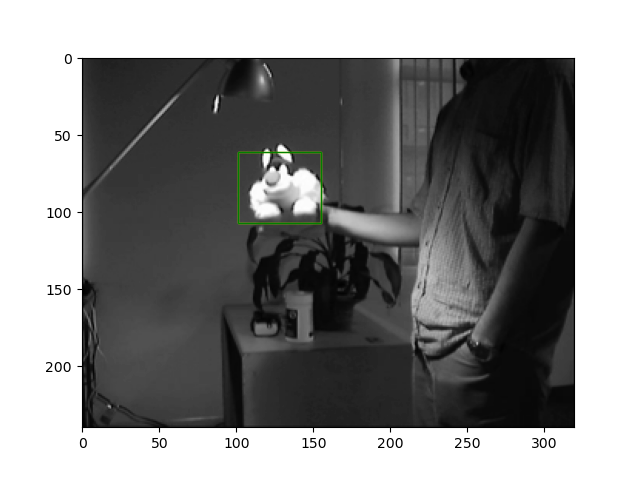
\includegraphics[width=\textwidth]{q2,3_frame0.png}
            \caption{Frame 0}
        \end{subfigure}
        \begin{subfigure}[b]{0.30\textwidth}
            \centering
            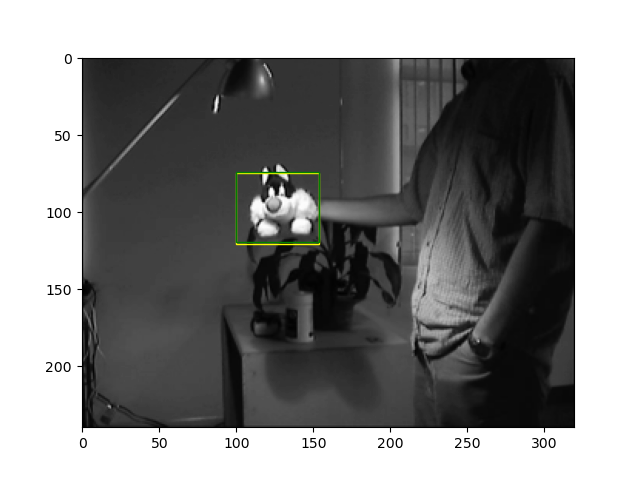
\includegraphics[width=\textwidth]{q2,3_frame100.png}
            \caption{Frame 100}
        \end{subfigure}
        \begin{subfigure}[b]{0.30\textwidth}
            \centering
            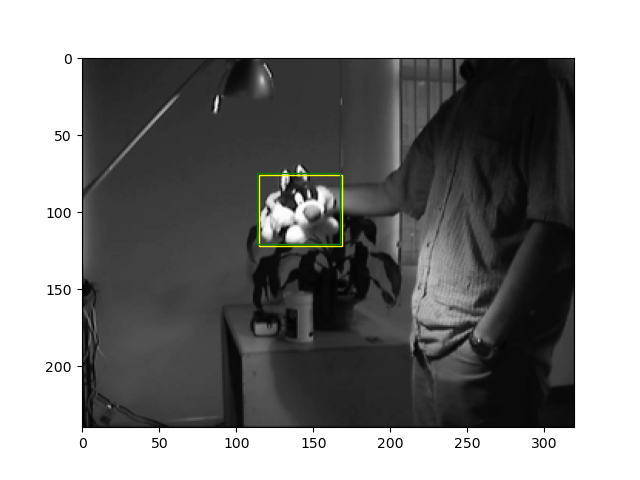
\includegraphics[width=\textwidth]{q2,3_frame200.png}
            \caption{Frame 200}
        \end{subfigure}
        \begin{subfigure}[b]{0.30\textwidth}
            \centering
            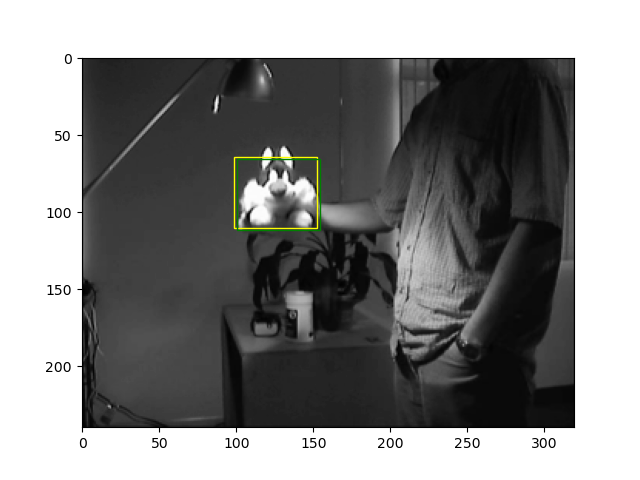
\includegraphics[width=\textwidth]{q2,3_frame300.png}
            \caption{Frame 300}
        \end{subfigure}
        \begin{subfigure}[b]{0.30\textwidth}
            \centering
            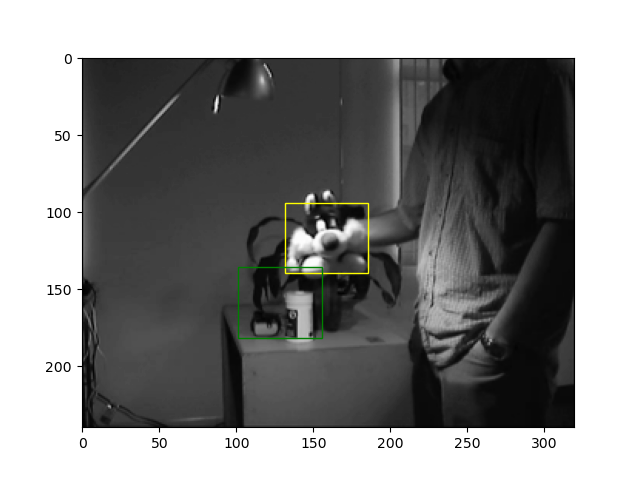
\includegraphics[width=\textwidth]{q2,3_frame400.png}
            \caption{Frame 400}
        \end{subfigure}
        \caption{Lucas-Kanade Tracking with Appearance Basis. The yellow bounding box is the result using appearance basis, and green one is the result with template correction.}
    \end{figure}

    \section{Affine Motion Subtraction}

    \subsection*{Q3.1}
    Here we present a derivation of the update step $\Delta p$.
    \medskip

    We are given the following wrap function:
    \begin{equation*}
    \mathcal{W}\left(x;p\right)=\left[\begin{array}{cc}
    1+p_{1} & p_{2}\\
    p_{4} & 1+p_{5}
    \end{array}\right]\left[\begin{array}{c}
    x\\
    y
    \end{array}\right]+\left[\begin{array}{c}
    p_{3}\\
    p_{6}
    \end{array}\right]=\left[\begin{array}{c}
    \left(1+p_{1}\right)x+p_{2}y+p_{3}\\
    p_{4}x+\left(1+p_{5}\right)y+p_{6}
    \end{array}\right]
    \end{equation*}
    Hence,
    \begin{align*}
    \frac{\partial \mathcal{W}\left(x;p\right)}{\partial p^{T}}=\begin{bmatrix}
    x & y & 1 & 0 & 0 & 0\\
    0 & 0 & 0 & x & y & 1
    \end{bmatrix}
    \end{align*}
    The objective function can be approixmated using first-order Taylor expansion:
    \begin{align*}
    &\arg \min _{\Delta p} \sum _{x}{\left| \left| \mathcal{I}_{t+1}\left(\mathcal{W}(x;p+\Delta p)\right)-\mathcal{I}_{t}\left(x\right)\right| \right| }_{2}^{2}\\
    =&\arg \min _{\Delta p} \sum _{x}{\left| \left| \mathcal{I}_{t+1}\left(x'\right)+\frac{\partial \mathcal{I}_{t+1}\left(x'\right)}{\partial x'^{T}}\frac{\partial \mathcal{W}\left(x;p\right)}{\partial p^{T}}\Delta p-\mathcal{I}_{t}\left(x\right)\right| \right| }_{2}^{2}\\
    =&\arg \min _{\Delta p} \sum _{x}{\left| \left| \frac{\partial \mathcal{I}_{t+1}\left(x'\right)}{\partial x'^{T}}\begin{bmatrix}
        x_{x} & x_{y} & 1 & 0 & 0 & 0\\
        0 & 0 & 0 & x_{x} & x_{y} & 1
    \end{bmatrix}\Delta p-\left(\mathcal{I}_{t}\left(x\right)-\mathcal{I}_{t+1}\left(x'\right)\right)\right| \right| }_{2}^{2}\\
    =&\arg \min _{\Delta p} \sum _{x}{\left| \left| \left[\begin{array}{ll}
        \left(\mathcal{I}_{t+1}\right)_{x}(x') & \left(\mathcal{I}_{t+1}\right)_{y}(x')
        \end{array}\right]\begin{bmatrix}
        x_{x} & x_{y} & 1 & 0 & 0 & 0\\
        0 & 0 & 0 & x_{x} & x_{y} & 1
    \end{bmatrix}\Delta p-\left(\mathcal{I}_{t}\left(x\right)-\mathcal{I}_{t+1}\left(x'\right)\right)\right| \right| }_{2}^{2}\\
    =&\arg \min _{\Delta p} \sum _{x}{\left| \left| D\Delta p-\left(\mathcal{I}_{t}\left(x\right)-\mathcal{I}_{t+1}\left(x'\right)\right)\right| \right| }_{2}^{2}\\ 
    =&\arg \min _{\Delta p} {\left| \left| A\Delta p-b\right| \right| }_{2}^{2}
    \end{align*}
    where $D=\left[\begin{array}{cccccc}
    \left(\mathcal{I}_{t+1}\right)_{x}\left(x'\right)x_{x} & \left(\mathcal{I}_{t+1}\right)_{x}\left(x'\right)x_{y} & \left(\mathcal{I}_{t+1}\right)_{x}\left(x'\right) & \left(\mathcal{I}_{t+1}\right)_{y}\left(x'\right)x_{x} & \left(\mathcal{I}_{t+1}\right)_{y}\left(x'\right)x_{y} & \left(\mathcal{I}_{t+1}\right)_{y}\left(x'\right)
    \end{array}\right]$. Now $A\in \mathbb{R}^{N\times 6}$.
    
    \textbf{Important Note:} The final affine transformation matrix outputted by the function will follow the conventions of $x$ being the horizontal axis and $y$ being the vertical axis, instead of the system used in \verb|scipy| where $x$ and $y$ are the first and second axis of the \verb|numpy| image array.
    \medskip

    This is the convention we are adopting: $\left[\begin{array}{ccc}1+p_{1} & p_{2} & p_{3}\\p_{4} & 1+p_{5} & p_{6}\end{array}\right]$.
    \medskip

    This is the convention for \verb|scipy|:$\left[\begin{array}{ccc}1+p_{5} & p_{4} & p_{6}\\p_{2} & 1+p_{1} & p_{3}\end{array}\right]$, which we are \textbf{NOT} using. 
    \medskip
    
    However, in \verb|SubtractDominantMotion|, we will convert the matrix using our convention to \verb|scipy|'s format. Refer to the code for more information.

    \subsection*{Q3.3}
    
    \begin{figure}[H]
        \centering
        \begin{subfigure}[b]{0.49\textwidth}
            \centering
            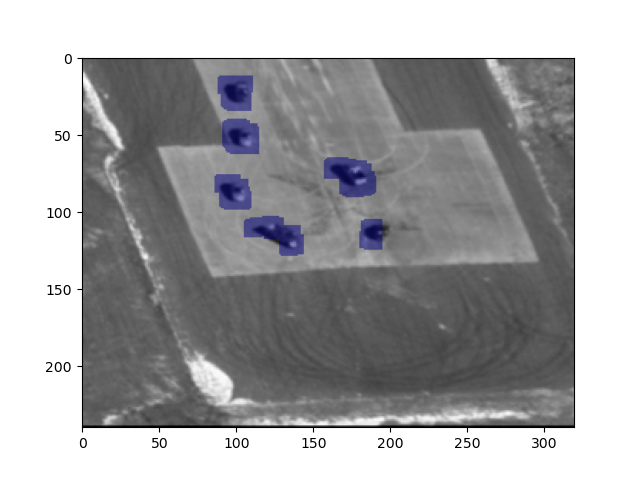
\includegraphics[width=\textwidth]{q3,3_frame30.png}
            \caption{Frame 30}
        \end{subfigure}
        \begin{subfigure}[b]{0.49\textwidth}
            \centering
            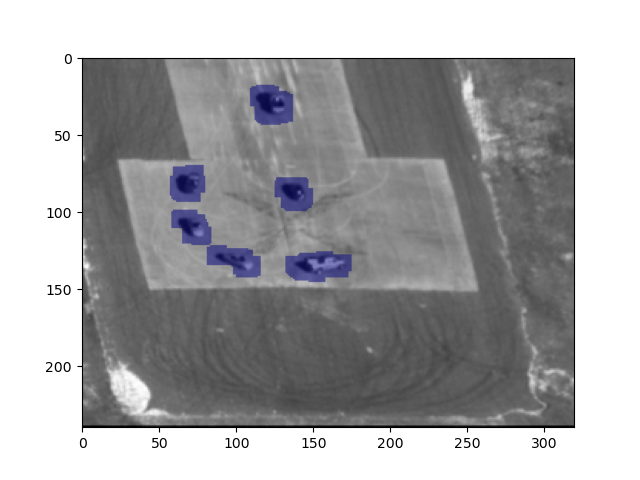
\includegraphics[width=\textwidth]{q3,3_frame60.png}
            \caption{Frame 60}
        \end{subfigure}
        \begin{subfigure}[b]{0.49\textwidth}
            \centering
            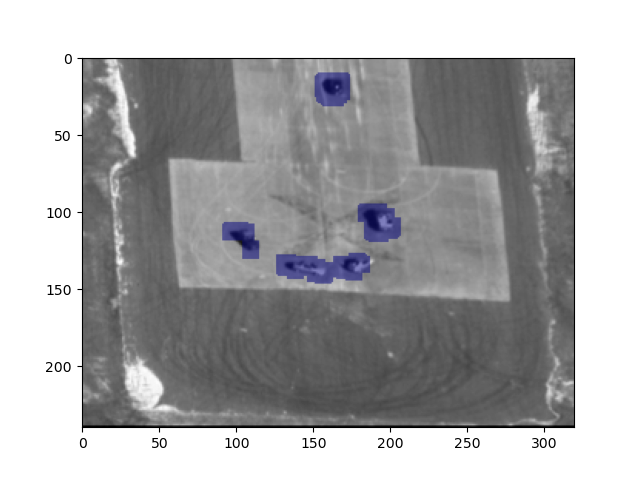
\includegraphics[width=\textwidth]{q3,3_frame90.png}
            \caption{Frame 90}
        \end{subfigure}
        \begin{subfigure}[b]{0.49\textwidth}
            \centering
            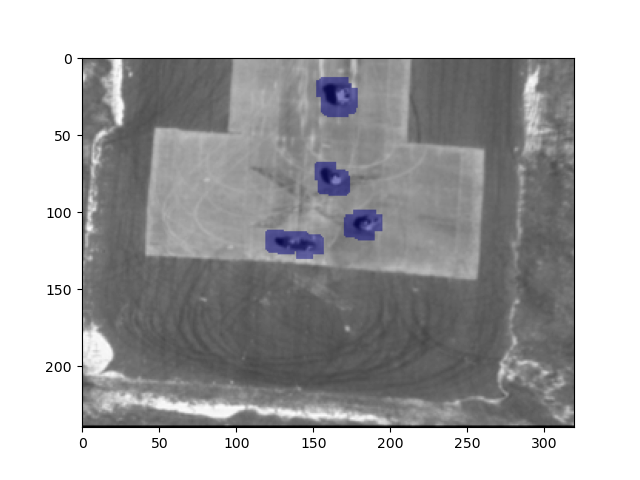
\includegraphics[width=\textwidth]{q3,3_frame120.png}
            \caption{Frame 120}
        \end{subfigure}
        \caption{Moving Object Detection using Dominant Motion Subtraction.}
    \end{figure}

    \section{Efficient Tracking}

    \subsection*{Q4.1}
    Before discussing its efficiency, we provide a derivation of the updating formula for the inverse compositional gradient descent.

    Using first-order Taylor expansion, we can approximate the image under an affine transformation with $\Delta p$:
    $$\mathcal{I}_{t}\left(\mathcal{W}\left(x;0+\Delta p\right)\right)\approx \mathcal{I}_{t}\left(\mathcal{W}\left(x;0\right)\right)+\frac{\partial \mathcal{I}_{t}\left(x\right)}{\partial x^{T}}\frac{\partial \mathcal{W}}{\partial p^{T}}\Delta p$$
    Basically, $\mathcal{I}_{t}\left(\mathcal{W}\left(x;0+\Delta p\right)\right)=\mathcal{I}_{t}\left(x\right)$. Hence, our objective function can be approximated as


    \begin{align*}
    &\sum _{x}{\left| \left| \mathcal{I}_{t}\left(\mathcal{W}\left(x;\Delta p\right)\right)-\mathcal{I}_{t+1}\left(\mathcal{W}\left(x;p\right)\right)\right| \right| }_{2}^{2}\\
    \approx&\sum _{x}{\left| \left| \mathcal{I}_{t}\left(\mathcal{W}\left(x;0\right)\right)+\frac{\partial \mathcal{I}_{t}\left(x\right)}{\partial x^{T}}\frac{\partial \mathcal{W}}{\partial p^{T}}\Delta p-\mathcal{I}_{t+1}\left(\mathcal{W}\left(x;p\right)\right)\right| \right| }_{2}^{2}\\
    =&\sum _{x}{\left| \left| \frac{\partial \mathcal{I}_{t}\left(x\right)}{\partial x^{T}}\begin{bmatrix}
    x_{x} & x_{y} & 1 & 0 & 0 & 0\\
    0 & 0 & 0 & x_{x} & x_{y} & 1
    \end{bmatrix}\Delta p-\left(\mathcal{I}_{t+1}\left(\mathcal{W}\left(x;p\right)\right)-\mathcal{I}_{t}\left(\mathcal{W}\left(x;0\right)\right)\right)\right| \right| }_{2}^{2}\\
    =&{\left| \left| A'\Delta p-b'\right| \right| }_{2}^{2}
    \end{align*}

    and our update rule is $\mathcal{W}\left(x;p\right)\leftarrow \mathcal{W}\left(x;p\right)\circ \mathcal{W}\left(x;\Delta p\right)^{-1}$. 
    \medskip

    This approach is computationally more efficient since the pseudoinverse of the $A'=\left(\dfrac{\partial \mathcal{I}_{t}\left(x_{i}\right)}{\partial {x}_{i}^{T}}\dfrac{\partial \mathcal{W}}{\partial p^{T}}\right)_{i}$ term in the inverse compositional method can be precomputed, while the $A=\left(\dfrac{\partial \mathcal{I}_{t+1}\left(x_{i}'\right)}{\partial {x}_{i}^{'T}}\dfrac{\partial \mathcal{W}}{\partial p^{T}}\right)_{i}$ in the classical approach has to be recalculated every time the $x'=x+p$ is updated in each iteration. Calculating inverse takes a lot of time, especially when the $A$s contains around 75k rows.
    \medskip

    To truly utilize the efficiency of precomputation, instead of selecting all points common to both images' valid area, we assume that the motion between two images are minimal and we only select points from a rectangle centered on the image. 
    \medskip
    
    Both versions of the affine matrix alignment are written in \verb|SubtractDominantMotion.py|. Uncomment the code to run each version. 

    \subsection*{Q4.2}

    The filter we want to obtain is given by $\displaystyle\arg \min _{g} {\sum }_{n=1}^{N}\frac{1}{2}{\left| \left| y_{n}-{x}_{n}^{T}g\right| \right| }_{2}^{2}$, or $\displaystyle\arg \min _{g} \frac{1}{2}{\left| \left| y-X^{T}g\right| \right| }_{2}^{2}+\frac{\lambda }{2}{\left| \left| g\right| \right| }_{2}^{2}$. Differentiate the objective function with respective to $g$ to find the minimum:
    \begin{align*}
    &\frac{\partial }{\partial g}\left(\frac{1}{2}{\left| \left| y-X^{T}g\right| \right| }_{2}^{2}+\frac{\lambda }{2}{\left| \left| g\right| \right| }_{2}^{2}\right)\\ =&-X\left(y-X^{T}g\right)+\lambda g\\ =&\left(XX^{T}+\lambda I\right)g-Xy\\ =&\left(S+\lambda I\right)g-Xy
    \end{align*}
    The minimum is attained when the gradient is zero:
    \begin{equation*}
    g^*=\left(S+\lambda I\right)^{-1}Xy
    \end{equation*}

    \subsection*{Q4.3}

    \begin{figure}[H]
        \centering
        \begin{subfigure}[b]{0.49\textwidth}
            \centering
            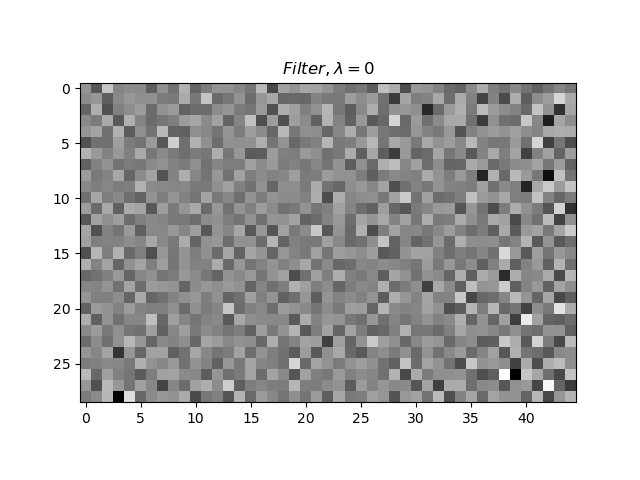
\includegraphics[width=\textwidth]{q43_filt0.png}
        \end{subfigure}
        \begin{subfigure}[b]{0.49\textwidth}
            \centering
            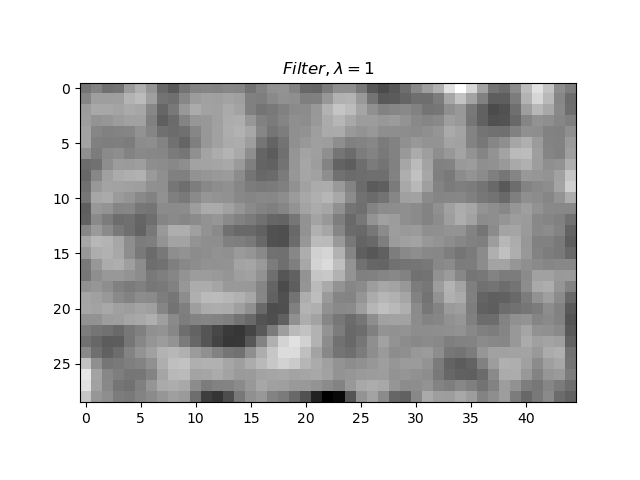
\includegraphics[width=\textwidth]{q43_filt1.png}
        \end{subfigure}
        \begin{subfigure}[b]{0.49\textwidth}
            \centering
            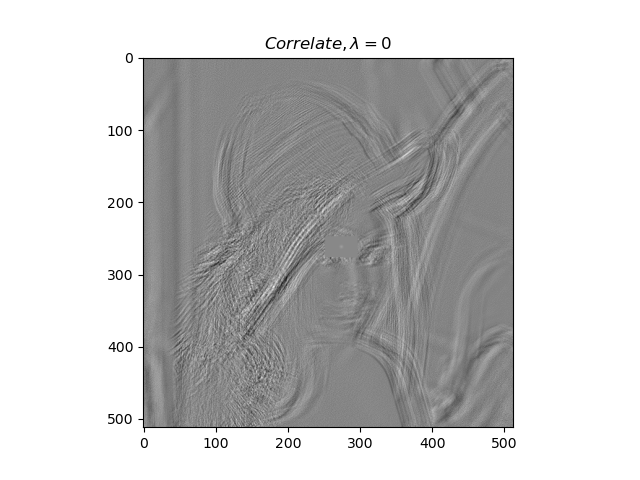
\includegraphics[width=\textwidth]{q43_img0.png}
        \end{subfigure}
        \begin{subfigure}[b]{0.49\textwidth}
            \centering
            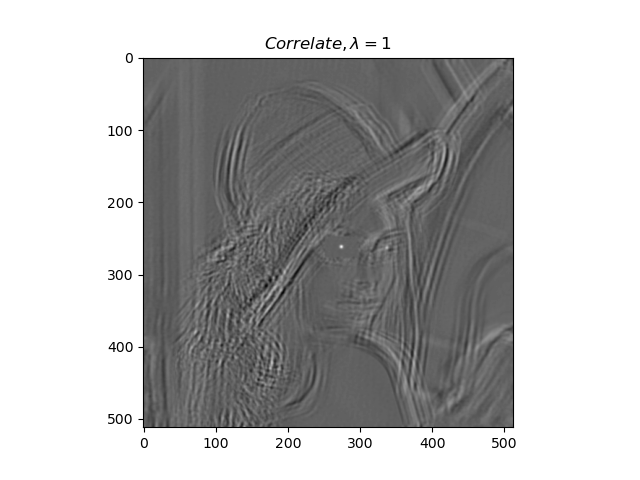
\includegraphics[width=\textwidth]{q43_img1.png}
        \end{subfigure}
        \caption{Linear discriminant weight vector and filter response under different regularization factors: $\lambda=0$ on the left and $\lambda=1$ on the right.}
    \end{figure}

    It should be emphasized that the motivation for correlation filters is to find a filter $g$, which will provides us with a desired response $y$ from a series of discriminators $x$ extracted from some part of the image. The performance we're trying to asses is how well the correlation filter gives us the desired response.
    \medskip

    Viewing the code, the desired response is $\exp (-{\left| \left| dp\right| \right| }_{2}^{2}/5)$, where ${\left| \left| dp\right| \right| }_{2}^{2}=dx^{2}+dy^{2}$ is the distance away from the center of Lena's eye; the less the distance, the stronger the response. This means that we want to fit a filter which gives a clear, strong response for an eye. Comparing the responses generated by the two correlation filters with different regularization, we find that $\lambda =1$ gives a strong response for the eye that we didn’t use for fitting $g$ (i.e. the eye on the right), while we only see random noise for $\lambda =0$.
    \medskip

    The reason for this is $\lambda =1$ gives more regularization than $\lambda =0$, preventing $g$ from straying away from the origin (the origin gives the default response, since the response to any image patch would evaluate to 0) and effectively preventing $g$ from overfitting to specifically the eye on the left. In other terms, $\lambda =1$ provides a trust region while $\lambda =0$ doesn’t.

    \subsection*{Q4.4}

    \begin{figure}[H]
        \centering
        \begin{subfigure}[b]{0.49\textwidth}
            \centering
            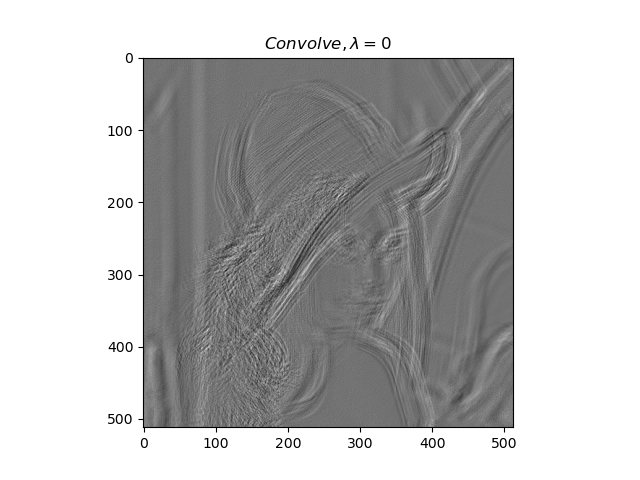
\includegraphics[width=\textwidth]{q44_img0.png}
        \end{subfigure}
        \begin{subfigure}[b]{0.49\textwidth}
            \centering
            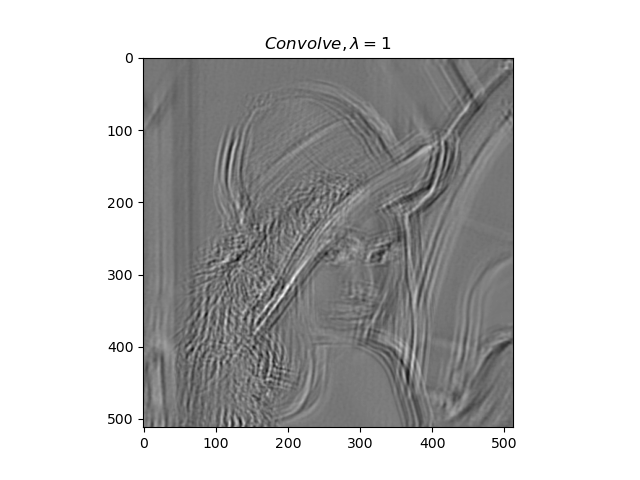
\includegraphics[width=\textwidth]{q44_img1.png}
        \end{subfigure}
        \begin{subfigure}[b]{0.49\textwidth}
            \centering
            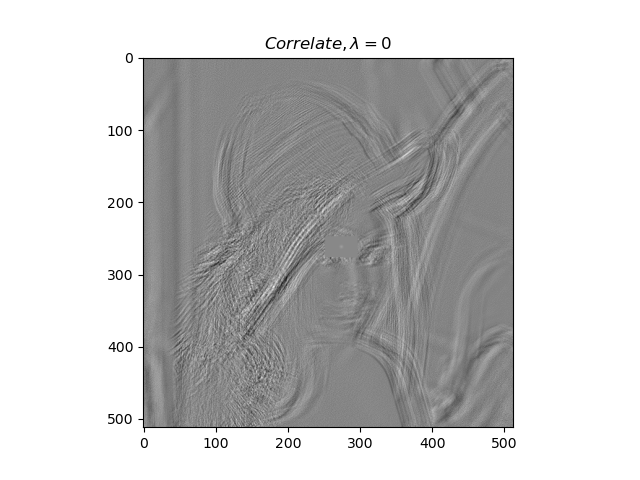
\includegraphics[width=\textwidth]{q43_img0.png}
        \end{subfigure}
        \begin{subfigure}[b]{0.49\textwidth}
            \centering
            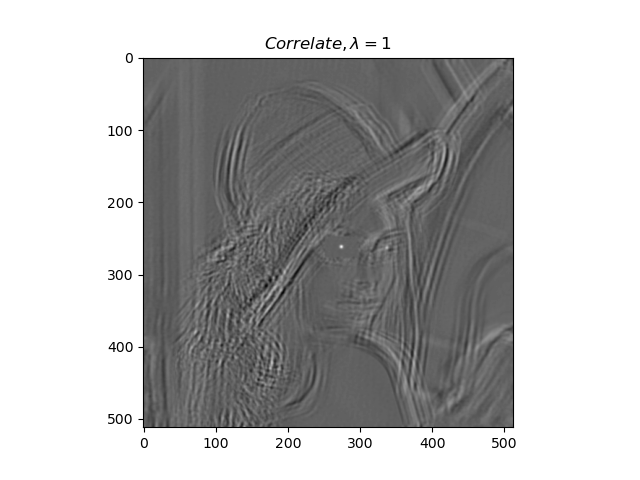
\includegraphics[width=\textwidth]{q43_img1.png}
        \end{subfigure}
        \caption{Image response under convolution (on the top) and correlation (on the bottom) using the same filter.}
    \end{figure}



    The response is different because convolution flips the filter horizontally and vertically before element-wise multiplication with the cropped image window, but correlation applies the given filter as it is. To get the same response as correlation using convolution, flip the filter before passing it into \verb|scipy.ndimage.convolve|, like \verb|filter[::-1,::-1]|. This means that the following two statements should give the same results:
    \medskip

    \centering
    \texttt{scipy.ndimage.correlate(img, filter)}
    \smallskip

    \centering
    \texttt{scipy.ndimage.convolve(img, filter{[}::-1,::-1{]})}
    
\end{document} % This is the end of the document